\section{Datasets and exploratory data analysis}

\subsection{Dataset}

Banking77 is downloaded from the public Hugging Face identifier \texttt{mteb/banking77} inside the notebook; no personal cloud drive is mounted. We use the official train~/~test split (9{,}993~/~3{,}076). Test data are never used for vocabulary fitting, PCA, early stopping, or model selection.

\begin{table}[H]
\centering
\caption{Banking77 corpus used in this study.}
\begin{tabular}{@{}llrrr@{}}
\toprule
Dataset & Hugging Face id & Classes & Train & Test \\
\midrule
Banking77 & \texttt{mteb/banking77} & 77 & 9{,}993 & 3{,}076 \\
\bottomrule
\end{tabular}
\end{table}

\subsection{Descriptive statistics}

Word counts use normalised text (lower case; HTML and URLs removed) and whitespace tokenization.

\begin{table}[H]
\centering
\caption{Descriptive statistics of Banking77 (training split unless noted).}
\small
\begin{tabular}{@{}lr@{}}
\toprule
Statistic & Value \\
\midrule
Training / test documents & 9{,}993 / 3{,}076 \\
Documents per class (min / max) & 35 / 187 \\
Balance ratio (min/max class count) & 0.187 \\
Words per document: mean (std) & 11.96 (7.89) \\
Median / 95th pct / 99th pct / max & 10 / 29.4 / 43 / 79 \\
Vocabulary with / without stop words & 2{,}353 / 2{,}128 \\
Share of tokens that are stop words & 60.7\% \\
Documents containing a negation & 25.5\% \\
\bottomrule
\end{tabular}
\end{table}

\begin{figure}[H]
\centering
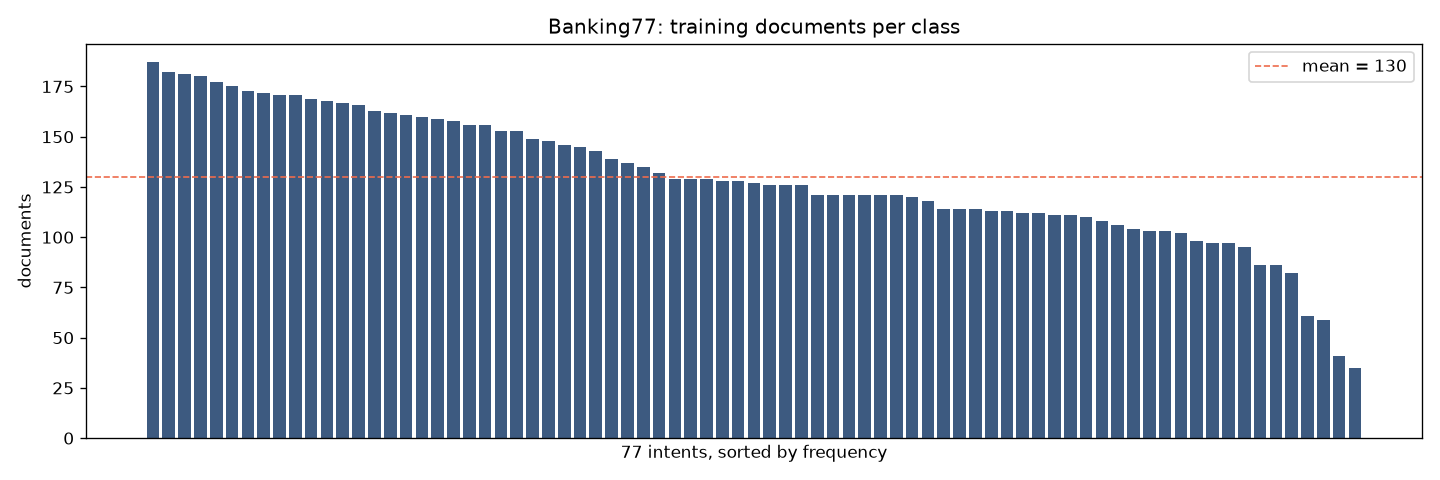
\includegraphics[width=0.72\textwidth]{banking77/class_balance.png}
\caption{Class balance of the Banking77 training set (ordered by frequency).}
\end{figure}

\begin{figure}[H]
\centering
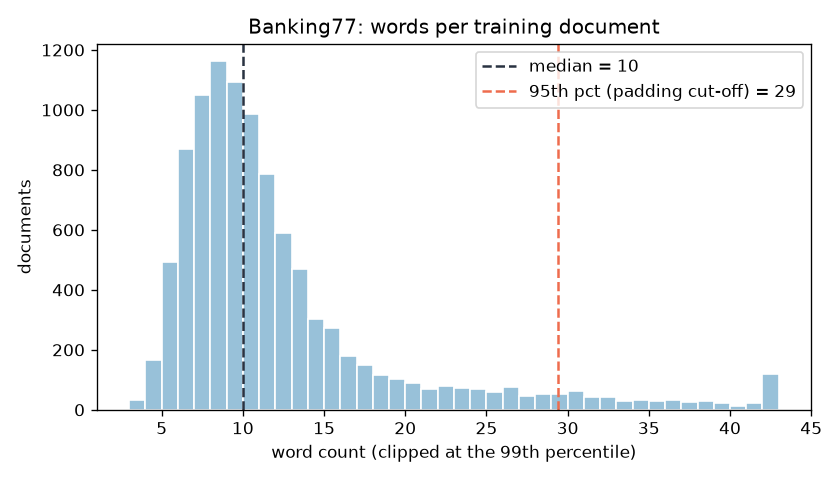
\includegraphics[width=0.72\textwidth]{banking77/length_hist.png}
\caption{Document length distribution with median and 95th-percentile cut-offs used for padding.}
\end{figure}

\begin{figure}[H]
\centering
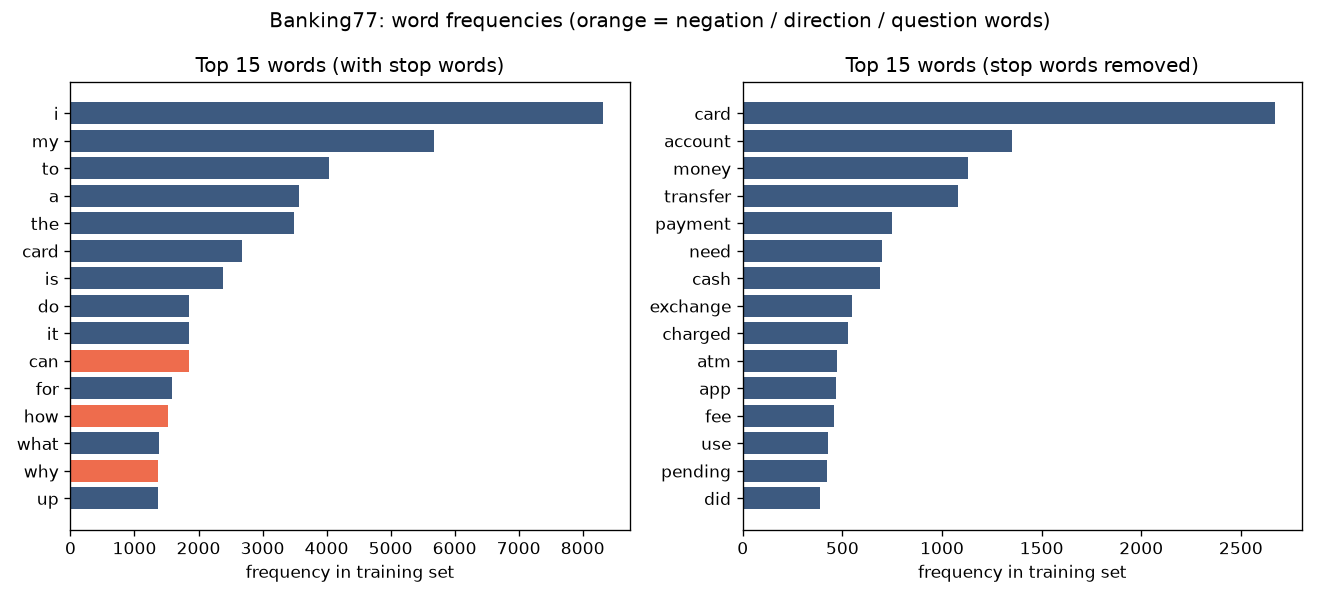
\includegraphics[width=0.88\textwidth]{banking77/top_words_comparison.png}
\caption{Top-15 words with and without stop words. Function words and question cues are frequent.}
\end{figure}

\subsection{Hypotheses derived from EDA}

\begin{itemize}
  \item \textbf{H1 (lexical overlap).} Intents share content nouns; unigram topic cues alone are insufficient, but TF-IDF bigrams and linear margins may still separate many classes.
  \item \textbf{H2 (function words matter).} Stop words comprise about 61\% of tokens and often encode intent (\textit{from}, \textit{into}, \textit{not}, \textit{why}, \textit{how}). Removing them should degrade TF-IDF and DistilBERT.
  \item \textbf{H3 (negation and state).} Negation appears in 25.5\% of training documents and frequently marks failure or pending states. Explicit negation marking should help static sequence models more than frozen contextual encoders.
  \item \textbf{H4 (length and padding).} Short queries (median 10 words) make truncation-to-10-tokens and unmasked padding particularly harmful for neural encoders; masked padding to the 95th percentile should improve Macro-F1 substantially for DistilBERT and BiLSTM.
\end{itemize}
